%        File: arfc-beamer.tex
%     Created: Sun May 5 10:00 PM 2013 C
%


%\documentclass[11pt,handout]{beamer}
\documentclass[9pt]{beamer}
\hypersetup{pdfpagemode=FullScreen}
\usetheme[white]{Illinois}
%\title[short title]{long title}
\title[MSR Transients]{Molten Salt Reactor Transients}
%\subtitle[short subtitle]{long subtitle}
\subtitle[]{How Power of The Future Performs In Accidents}
%\author[short name]{long name}
\author[Gavin Ridley]{Gavin Ridley, Dr. Alex Lindsay, Prof. Kathryn Huff\\Advanced Reactors and Fuel Cycles Group}
%\date[short date]{long date}
\date[07.20.2017]{07.20.2017}
%\institution[short name]{long name}
\institute[UIUC]{University of Illinois at Urbana-Champaign}

%\usepackage{bbding}
%
\usepackage{mathtools}
\usepackage{commath}
\usepackage{amsfonts}
\usepackage{amsmath}
\usepackage{xspace}
\usepackage{graphicx}
\usepackage{subfigure}
\usepackage{booktabs} % nice rules for tables
\usepackage{microtype} % if using PDF
\usepackage{bigints}
\usepackage{minted}
\usepackage{tikz}
\usepackage{animate}

\newcommand{\units}[1] {\:\text{#1}}%
\newcommand{\SN}{S$_N$}%{S$_\text{N}$}%{$S_N$}%
\DeclareMathOperator{\erf}{erf}
%I need some complimentary error funcitons... 
\DeclareMathOperator{\erfc}{erfc}
%page numbers
\setbeamertemplate{footline}[page number]
\setbeamertemplate{caption}[numbered]
%Those icons in the references are terrible looking
\setbeamertemplate{bibliography item}[text]

%%% Functions and environments from user:
% some functions and environments that will be useful
%
%%% An imageframe has one fullscreen image as background
%%% and maybe some text on top.
\newenvironment{imageframe}[1]
{
\setbeamertemplate{background}{%
\parbox[c][\paperheight]{\paperwidth}{%
\includegraphics[width=\paperwidth,height=\paperheight]{#1}
}}
\begin{frame}
  \color{white}
  }{\end{frame}}


%%% A wordframe has one word (or few) big and centered
\newenvironment{wordframe}
{
\begin{frame}
  \bf\usebeamerfont{word frame}
  }{\end{frame}}


%%% A defnframe defines a word or phrase
\newenvironment{defnframe}[1]
{
\begin{frame}
  \usebeamerfont{title}\usebeamercolor[fg]{box title}\Large #1: \\
  \vskip0.7cm
  \usebeamercolor[fg]{normal text}\Large\itshape
  }{\end{frame}}

\newcommand{\emptyslide}{\begin{frame}[plain]\end{frame}}


%%%% Acronym support

\usepackage[acronym,toc]{glossaries}
\include{acros}

\makeglossaries

%try to get rid of header on title page\dots
\makeatletter
    \newenvironment{withoutheadline}{
        \setbeamertemplate{headline}[default]
        \def\beamer@entrycode{\vspace*{-\headheight}}
    }{}
\makeatother

\begin{document}
%%%%%%%%%%%%%%%%%%%%%%%%%%%%%%%%%%%%%%%%%%%%%%%%%%%%%%%%%%%%%
%% From uw-beamer Here's a handy bit of code to place at 
%% the beginning of your presentation (after \begin{document}):
\newcommand*{\alphabet}{ABCDEFGHIJKLMNOPQRSTUVWXYZabcdefghijklmnopqrstuvwxyz}
\newlength{\highlightheight}
\newlength{\highlightdepth}
\newlength{\highlightmargin}
\setlength{\highlightmargin}{2pt}
\settoheight{\highlightheight}{\alphabet}
\settodepth{\highlightdepth}{\alphabet}
\addtolength{\highlightheight}{\highlightmargin}
\addtolength{\highlightdepth}{\highlightmargin}
\addtolength{\highlightheight}{\highlightdepth}
\newcommand*{\Highlight}{\rlap{\textcolor{HighlightBackground}{\rule[-\highlightdepth]{\linewidth}{\highlightheight}}}}
%%%%%%%%%%%%%%%%%%%%%%%%%%%%%%%%%%%%%%%%%%%%%%%%%%%%%%%%%%%%%
%%--------------------------------%%
\begin{withoutheadline}
\frame{
  \titlepage
}
\end{withoutheadline}

%%--------------------------------%%
\AtBeginSection[]{
\begin{frame}
  \frametitle{Outline}
  \tableofcontents[currentsection]
\end{frame}
}

\section{Motivation}
\subsection{Molten Salt Reactors}
\begin{frame}
    \frametitle{Energy for the future}
        \begin{columns}
            \column[t]{5cm}

            \begin{quote}
                    Cheap and abundant nuclear energy is no longer a luxury; it will eventually be a necessity for the maintenance of the human condition. -- Alvin Weinberg
            \end{quote}

            %From \textit{The Age of Substitutability} by Goeller and Weinberg: energy is the ultimate limiting resource of future society.

            \begin{center}
                    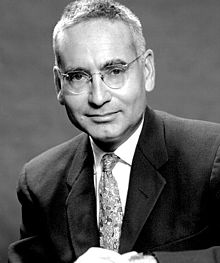
\includegraphics[height=0.3\textheight]{weinberg}
            \end{center}
            \column[t]{5cm}

            Molten salt reactors offer a convincing solution to the problem of fossil fuels.

            \begin{itemize}
                \item{Potentially much cheaper than normal nuclear}
                \item{Make meltdowns impossible}
                \item{Better natural resource utilization}
            \end{itemize}

        \end{columns}
\end{frame}

\begin{frame}
  \frametitle{MSR Comparison}
  
  \begin{columns}
      \column[t]{5cm}
      \textbf{Topaz Solar Farm}

      \begin{itemize}
          \item{9.5 sq. mi of California desert}

          \item{Max output of 550 MW(e), on average makes 132 MW(e)}

          \item{\$2.5B construction}
      \end{itemize}

      \begin{figure}[h]
          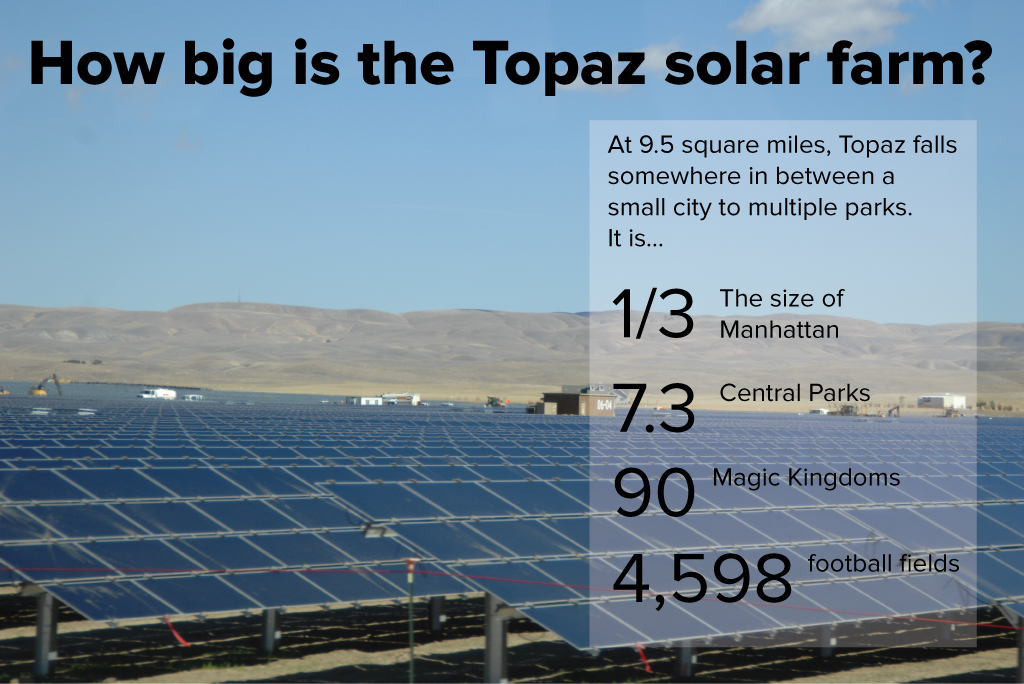
\includegraphics[width=\textwidth]{topaz}
          \caption{Topaz solar farm in California, credit GigaOM media}
      \end{figure}

      \column[t]{5cm}
      \textbf{Terrestrial Energy IMSR concept}

      \begin{itemize}
          \item{About 300 MW(e) output, more than double Topaz farm}

          \item{Initial cost estimates rank IMSR cheaper than coal}
      \end{itemize}
      \begin{figure}[h]
          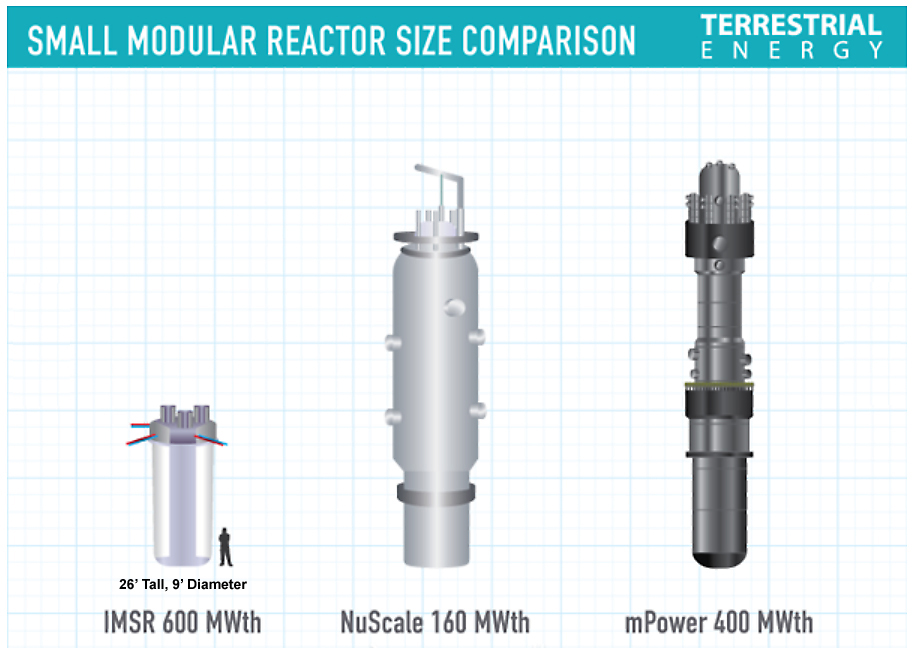
\includegraphics[width=\textwidth]{IMSR}
          \caption{IMSR and some other small nuclear designs, credit Terrestrial Energy}
      \end{figure}
  \end{columns}

\end{frame}

\subsection{What We Simulated}
\begin{frame}
    \frametitle{Benchmark Case: MSRE}
        \begin{columns}
            \column[t]{5cm}
            \begin{itemize} 
                \item{Constructed at Oak Ridge National Lab, ran reliably 1965-1969 at 7.4 MW(th)}


                \item{Various tests proved theory and tech-readiness for full-scale power plants}


                \item{Stopped operation since all needed experiments were done}
            \end{itemize}

            \column[t]{5cm}
            \begin{figure}[h]
            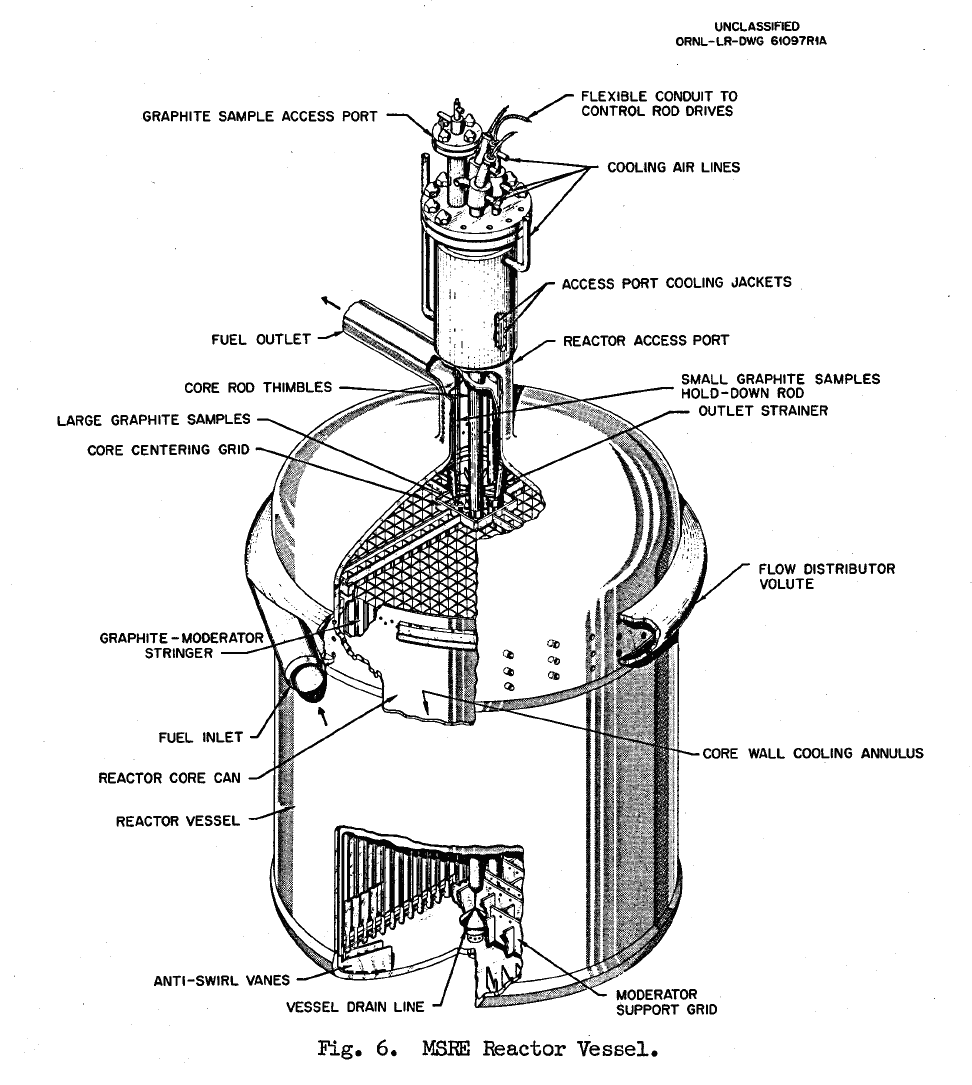
\includegraphics[width=\textwidth]{msreCore}
            \caption{MSRE reactor core diagram from ORNL technical reports}
        \end{figure}
        \end{columns}
\end{frame}

%\imageframe{msrePlant}

\begin{imageframe}{msrePlant}
\end{imageframe}
\begin{frame}
  \frametitle{MSRs: An Intrinsically Coupled System I}
      \textbf{Neutrons'}
      %\begin{equation}
      %\begin{aligned}
      %    \frac{1}{v(E)} \pd{\psi}{t} + \hat{\Omega}\cdot \nabla \psi + \textcolor{red}{\Sigma_t} \psi =& \frac{\chi_p(E)}{4 \pi} \int_{0}^{\inf} \nu_p(E') \textcolor{red}{\Sigma_f} \phi dE' + \sum_i \frac{\chi_d(E)}{4 \pi} \lambda _i C_i + \\
      %                                                                                                  & \int_{4\pi}  \int_{0}^{\inf} \textcolor{red}{\Sigma_s(E'\rightarrow E,\hat{\Omega}'\rightarrow \hat{\Omega})} \psi dE' d\hat{\Omega}\\
      %\end{aligned}
      %\end{equation}
      changing concentrations can be described approximately with coupled diffusion equations:
		%% \frac{1}{v_g}\frac{\partial \phi_g}{\partial t} - \nabla \cdot D_g \nabla \phi_g
		%% + \Sigma_g^r \phi_g = \sum_{g \ne g'}^G \Sigma_{g'\rightarrow g}^s \phi_{g'} + \chi_g^p \sum_{g' = 1}^G (1 - \beta)
		%% \nu \Sigma_{g'}^f \phi_{g'}
\begin{equation}
				\frac{1}{v_g}\frac{\partial \phi_g}{\partial t}   = \nabla \cdot D_g
				\nabla \phi_g +
				\sum_{g \ne g'}^G
				\Sigma_{g'\rightarrow g}^s \phi_{g'} + \chi_g^p \sum_{g' = 1}^G (1 -
				\beta) \nu \Sigma_{g'}^f \phi_{g'} + \chi_g^d \sum_i^I \lambda_i C_i - \Sigma_g^r \phi_g
		\label{eq:neutrons}
\end{equation}
				where
				$v_g    $    = \mbox{speed of neutrons in group g} \\
				$\phi_g $    = \mbox{flux of neutrons in group g} \\
				$t      $    = \mbox{time} \\
				$D_g    $    = \mbox{Diffusion coefficient for neutrons in group g} \\
				$\Sigma_g^r$ = \mbox{macroscopic cross-section for removal of neutrons
				from group g} \\
				$\Sigma_{g'\rightarrow g}^s$ = \mbox{macroscopic cross-section of
				scattering from g' to g} \\
				$\chi_g^p$   = \mbox{prompt fission spectrum, neutrons in group g} \\
				$G$          = \mbox{number of discrete groups, g} \\
				$\nu$        = \mbox{number of neutrons produced per fission} \\
				$\Sigma_g^f$ = \mbox{macroscopic cross section for fission due to neutrons in group g} \\
				$\chi_g^d$   = \mbox{delayed fission spectrum, neutrons in group g} \\
				$I $         = \mbox{number of delayed neutron precursor groups} \\
				$\beta $     = \mbox{delayed neutron fraction}\\
				$\lambda_i $ = \mbox{average decay constant of delayed neutron precursors
				in precursor group i} \\
				$C_i $       = \mbox{concentration of delayed neutron precursors in precursor
				group i} .
\end{frame}

\begin{frame}
    \frametitle{MSRs: An Intrinsically Coupled System II}
    \textbf{Delayed neutron precursors} are products of freshly split uranium that emit a new neutron after a delay.
    \textit{critical} to reactor control; they shift power change timescales from picoseconds to seconds despite
    only being a few tenths of a percent of emitted neutrons.

	\begin{equation}
			\frac{\partial C_i}{\partial t} = \sum_{g'= 1}^G \beta_i \nu
			\Sigma_{g'}^f \phi_{g'} - \lambda_i C_i - \frac{\partial}{\partial z} u
			C_i \label{eq:precursors}
	\end{equation}

    % note, flow is primarily only the +z direction

    \textbf{Heat and temperature} affect the coefficients in Equation \ref{eq:neutrons} significantly. Energy conservation must be solved:

\begin{equation}
        \rho_fc_{p,f}\frac{\partial T_f}{\partial t} + \nabla\cdot\left(\rho_f
        c_{p,f} \vec{u}\cdot T_f -k_f\nabla T_f\right) =  Q_f
  \label{eq:fuel_temp}
\end{equation}

\begin{tabular}{cc}
  $\rho_f $ &= \mbox{density of fuel salt}\\
  $c_{p,f}$ &= \mbox{specific heat capacity of fuel salt}\\
  $T_f    $ &= \mbox{temperature of fuel salt}\\
  $\vec{u}$ &= \mbox{velocity of fuel salt}\\
  $k_f    $ &= \mbox{thermal conductivity of fuel salt}\\
  $Q_f    $ &= \mbox{source term}\\
\end{tabular}

\end{frame}

\subsection{Multiphysics Coupling}
\section{Methods}
\subsection{MOOSE}
\begin{imageframe}{moose}
\end{imageframe}
\begin{frame}
\frametitle{MOOSE Physics Representation}
  \begin{itemize}
      \item{Highly object-oriented code solves weak form of PDE using finite element method}
      \item{PETSc solves resulting system of nonlinear equations using generalized minimal residual method (GMRES)}
      \item{Some of the world's most cutting-edge numerical algorithms and scalable parallel computing are made painlessly accessible to the everyday user}
	\end{itemize}

\end{frame}

\begin{frame}[fragile]
    \frametitle{MOOSE Example}
    In MOOSE, the term $D \nabla^2 u$ is easily represented by:
  \begin{minted}{c++}
Real
GroupDiffusion::computeQpResidual()
{
  return _D[_qp][_group] * _grad_test[_i][_qp] *
         computeConcentrationGradient(_u, _grad_u, _qp);
}

  \end{minted}

  A vacuum boundary condition in neutronics calculations can easily be represented by:
  \begin{minted}{c++}
Real
VacuumConcBC::computeQpResidual()
{
  return _test[_i][_qp] * computeConcentration(_u, _qp) / 2.;
}
  \end{minted}

\end{frame}

\subsection{Sustainable, open software}
\begin{frame}
  \frametitle{Moltres}
  \begin{columns}
  \column[t]{5cm}
  \begin{itemize}
  \item{\textcolor{blue}{github.com/arfc/moltres}}
  \item{Publicly developed on github}
  \item{Continuous integration by Civet}
  \item{Includes detailed guide for contributing}
  \end{itemize}

  \textbf{Most importantly:} physics kernels, boundary conditions, and even capability to couple
  into MOOSE Navier-Stokes solvers provided to the moltres user


  \column[t]{5cm}

  
\includegraphics[width=\textwidth]{moltres}

  \end{columns}
\end{frame}

\subsection{Group Constant Generation}
\begin{frame}
  \frametitle{Group constant generation}
    \begin{columns}

    \column[t]{5cm}

    \column[t]{3.7cm}
    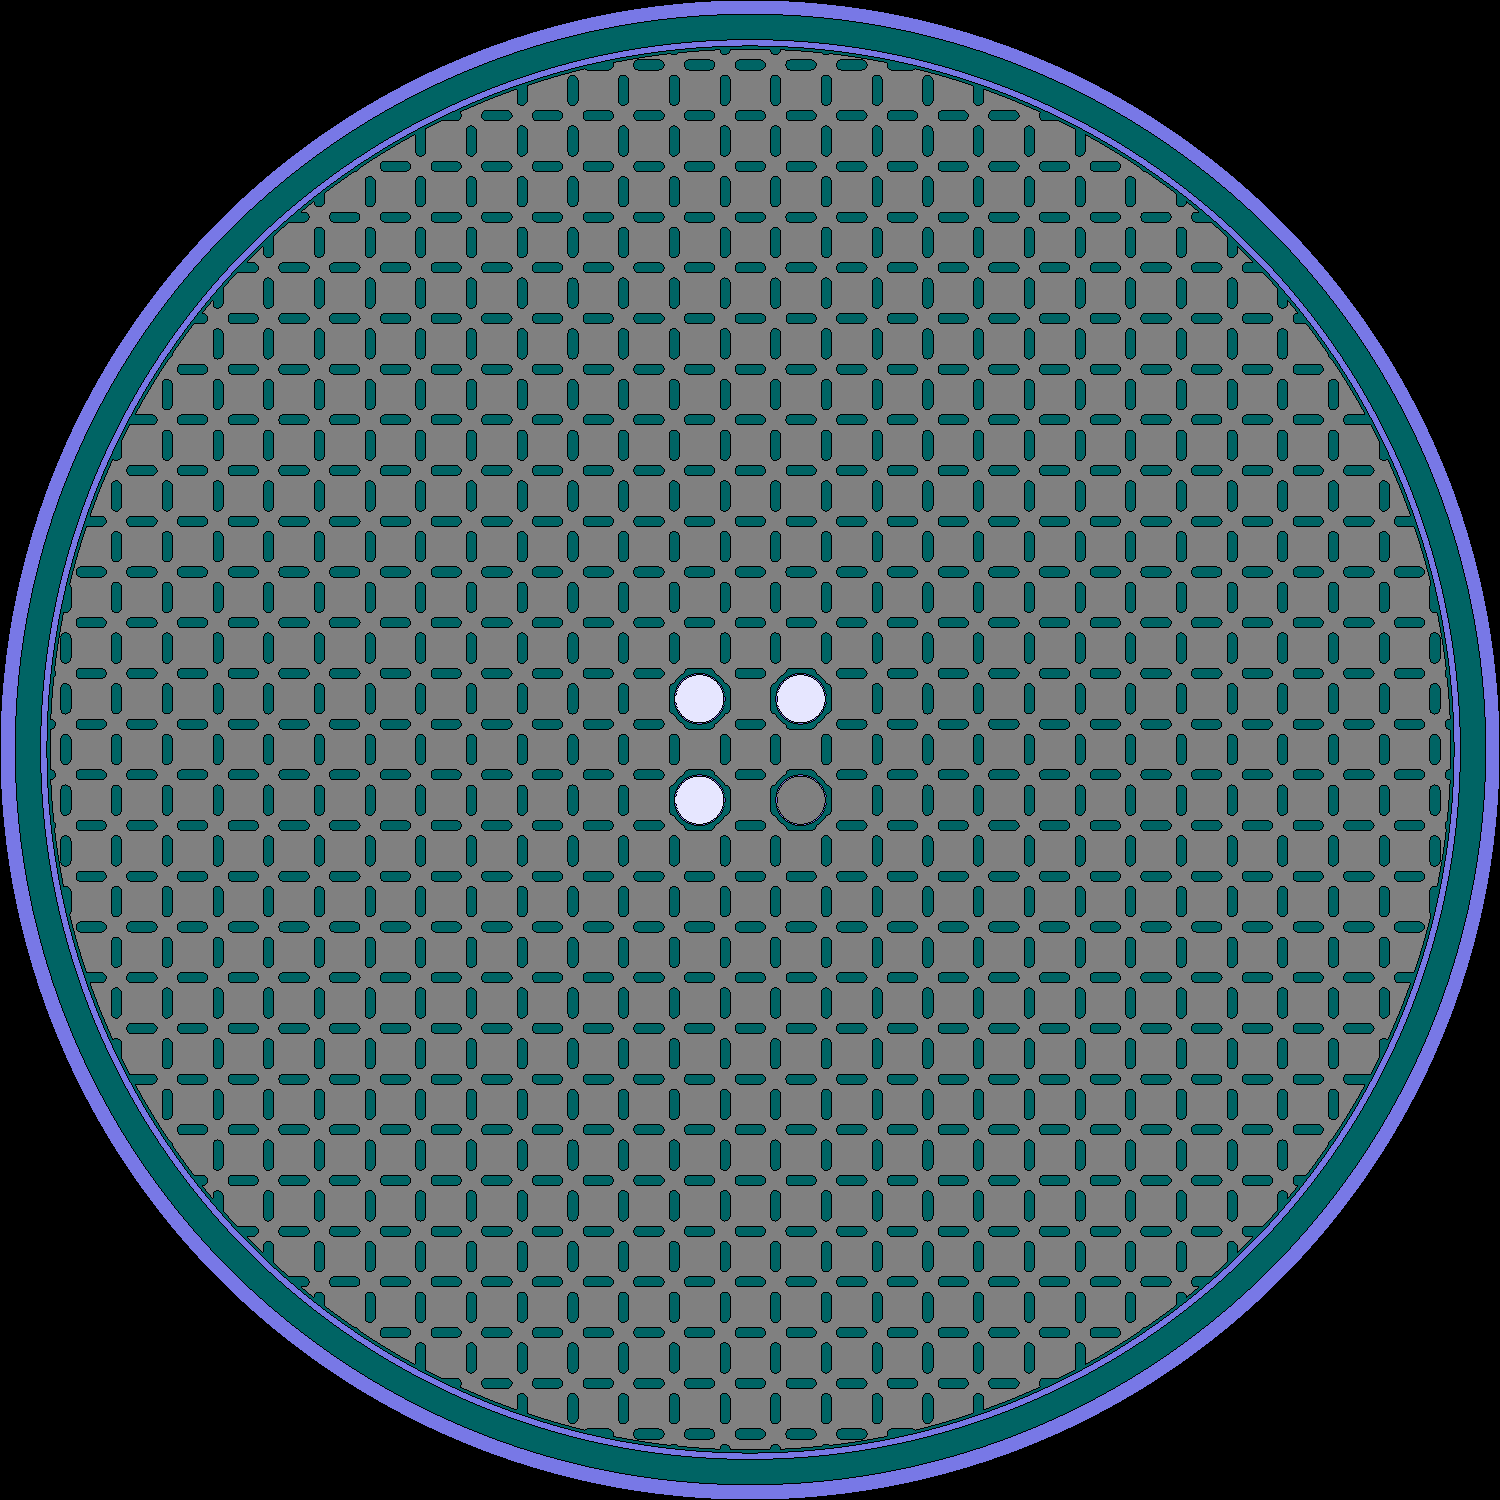
\includegraphics[width=\textwidth]{msregeom}

    
\includegraphics[width=\textwidth]{msremesh}

    \end{columns}


\end{frame}

\section{Results \& Conclusion}
\begin{frame}
  \frametitle{Results}
  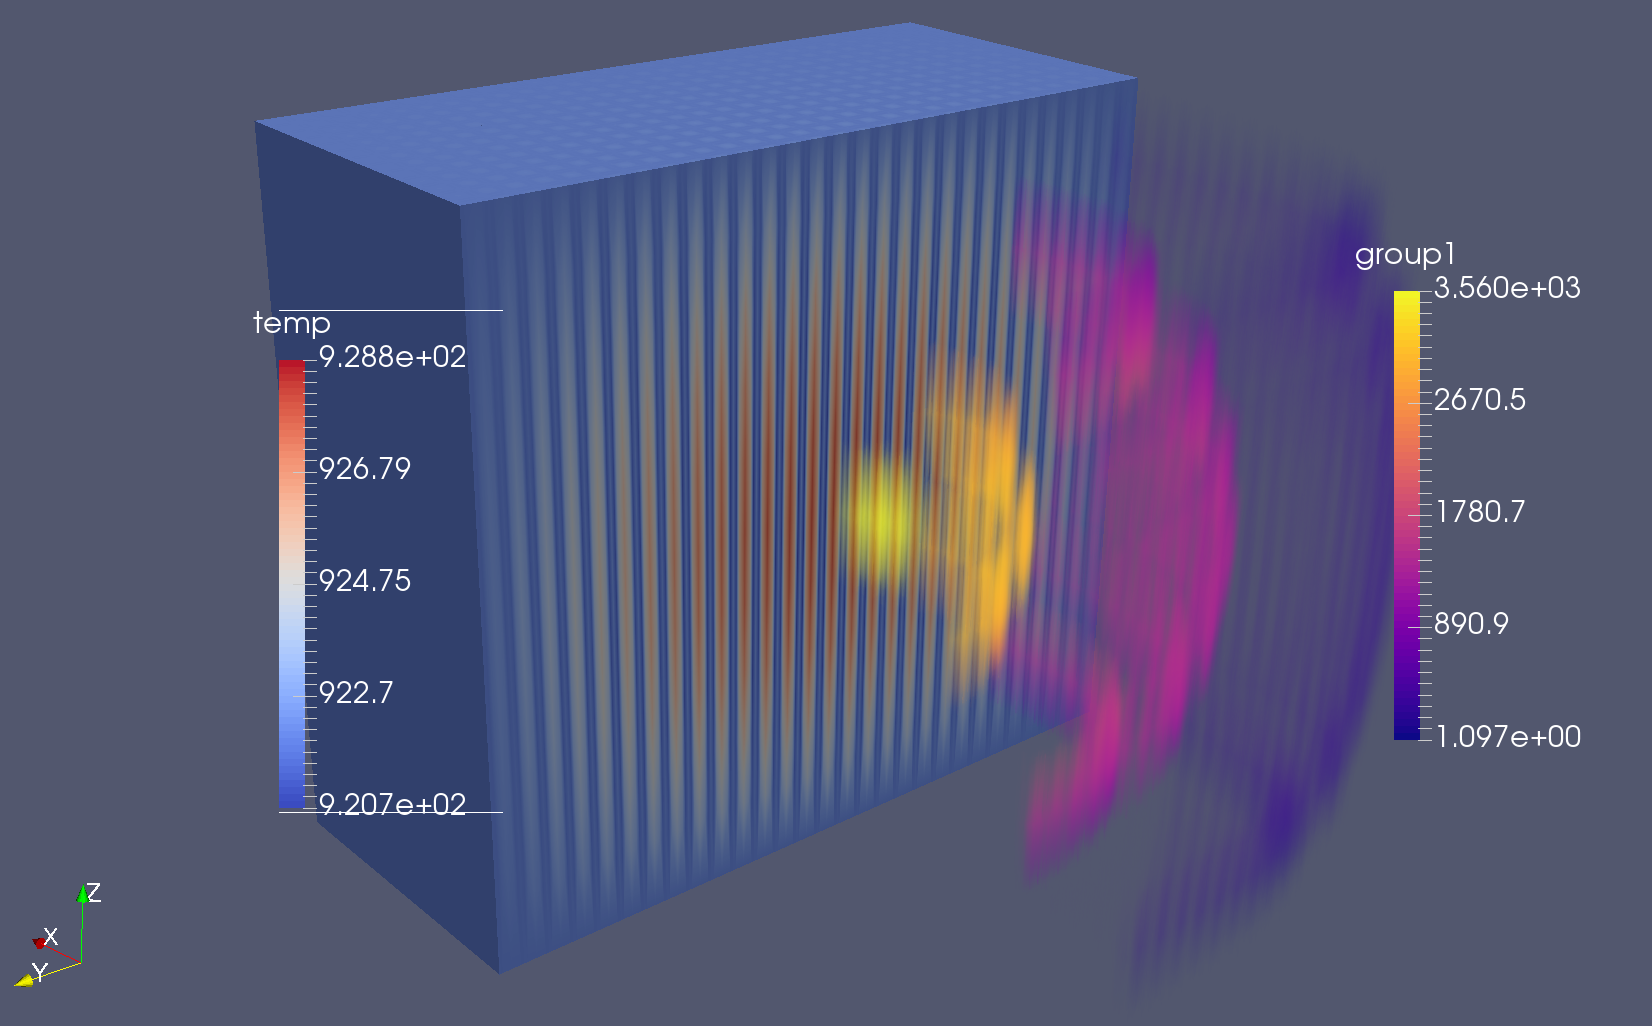
\includegraphics[width=\textwidth]{cuboidal}
\end{frame}

\begin{frame}
    \frametitle{More Results}
    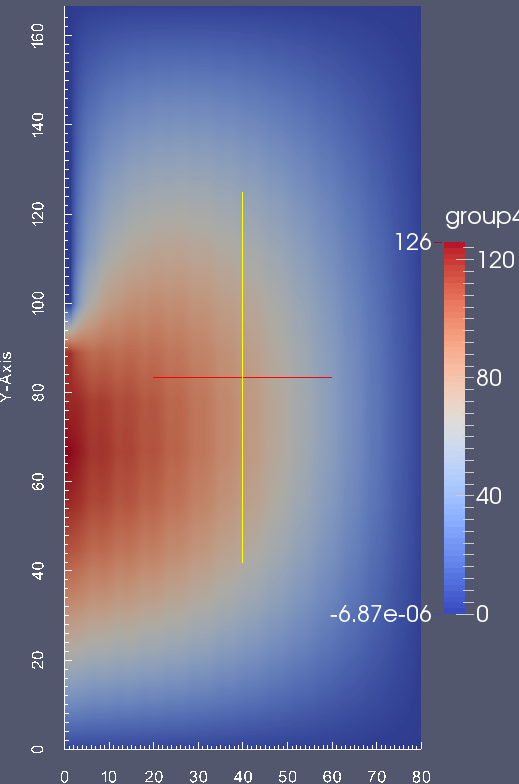
\includegraphics[height=\textheight]{rodded}

\end{frame}

\begin{frame}
  \frametitle{Conclusion}
        Moltres can contribute to building power for the future.
        \begin{itemize}
                \item Group constants generated for MSRE-like reactors, made public on github
                \item Work in progress to automatically model salt heat exchangers, salt loops
        \end{itemize}

        \textbf{Future work}
        \begin{itemize}
            \item Will build small research reactors, transport effects may dominate
            \item $\quad$ $\implies$ implement $P_3$ or so transport
            \item Include molten salt-specific thermalhydraulics models
        \end{itemize}



\end{frame}

\begin{frame}
  \frametitle{Acknowledgement}
        Acknowledgements go to Dr. Alex Lindsay, Dr. Kathryn Huff for the outstading help and support.
        This project was funded by the NCSA REU INCLUSION program.
    \end{frame}


{ % all template changes are local to this group.
    \setbeamertemplate{navigation symbols}{}
    \begin{frame}[plain]
        \begin{tikzpicture}[remember picture,overlay]
            \node[at=(current page.center)] {
                    \vspace{5cm}
                
\includegraphics[width=\paperwidth]{nucular}
            };
        \end{tikzpicture}
     \end{frame}
}
%%--------------------------------%%
%%--------------------------------%%
%\begin{frame}[allowframebreaks]
%  \frametitle{References}
%  \bibliographystyle{plain}
%  {\footnotesize \bibliography{bibliography.bib} }
%
%\end{frame}

%%--------------------------------%%


\end{document}



